%!TEX root = ../report.tex
\documentclass[report.tex]{subfiles}
\begin{document}
    \chapter{Evaluation and Results}

    \section{Experiment Description}

    Describe the experiments/evaluation you are performing to analyse your method.
    \begin{itemize}
        \item Short note on the experiment setup
        \item Short note on the evaluation metrics
        \item The folder structure
    \end{itemize}
        \begin{itemize}
    \item We are using BOP YCBV dataset(\href{https://bop.felk.cvut.cz/datasets/}{BOP YCBV}) for our evaluation purpose as we have ground truth information about the object pose and the camera pose. We will be performing the evaluation on test scene 000048 of BOP YCBV dataset. There are only 5 unique objects in the scene and there are 2243 camera poses and images.
    
\begin{figure}[H]
\centering
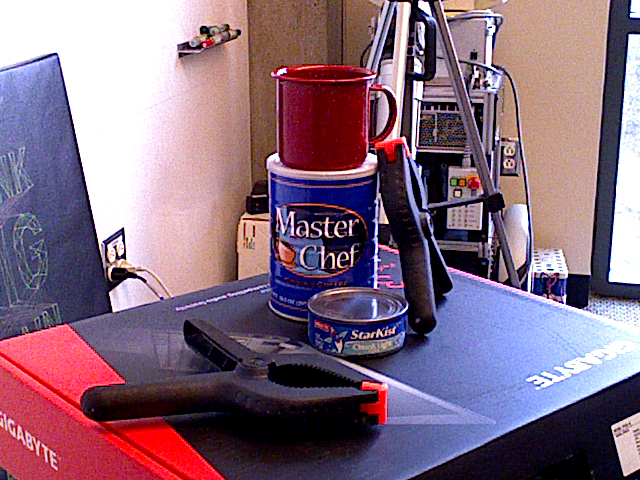
\includegraphics[width=0.8\textwidth] {Images/scene48.png}
\caption{\centering Sample image from Scene 000048 of BOP YCBV dataset}
\label{fig:scene48}
\end{figure}

    \item In BOP YCBV dataset, there are RGB and depth images. Also, 3 json files are present. scene\_gt.json contains the object poses in terms of rotation and translation matrix for each object in a particular image. scene\_camera.json contains the intrinsic and extrinsic parameters of the camera in each image. scene\_gt\_info.json contains the bounding box parameters for each object in each image. The bounding box parameters are in the format (x, y, width, height) where x,y is the top left corner. More details about the dataset format is given in the project website.(\href{https://github.com/thodan/bop\_toolkit/blob/master/docs/bop\_datasets\_format.md}{format})
\end{itemize}

\subsubsection{Iterative optimization}
\begin{itemize}

\begin{figure}[H]
\centering
\begin{minipage}{.45\textwidth}
  \centering
  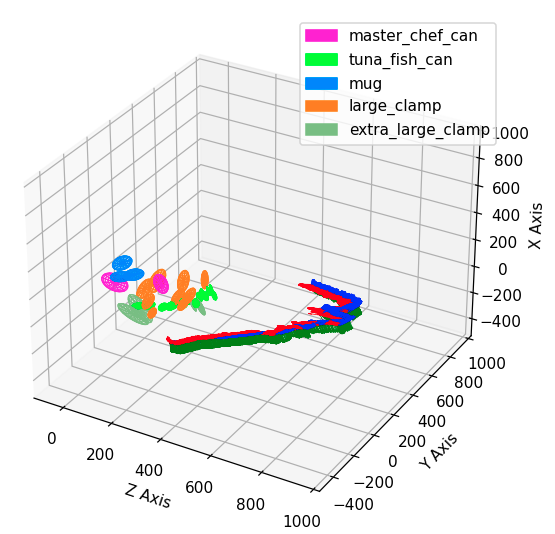
\includegraphics[width=\textwidth]{Images/iter_box_traj.png}
  \captionof{figure}{Iterative optimized trajectory and object ellipsoids}
  \label{fig:iterative_48}
\end{minipage}%
\begin{minipage}{.45\textwidth}
  \centering
  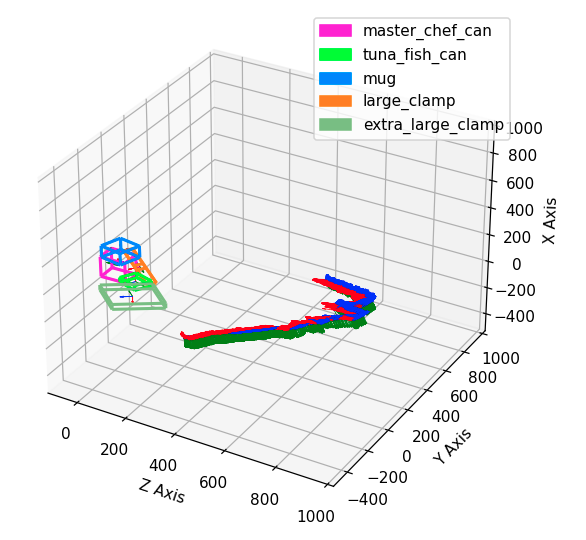
\includegraphics[width=\textwidth]{Images/48_gt_traj_box.png}
  \captionof{figure}{Ground truth trajectory and object 3D box}
  \label{fig:ground_truth_48}
\end{minipage}
\end{figure}

\begin{figure}[H]
\centering
\begin{minipage}{.45\textwidth}
  \centering
  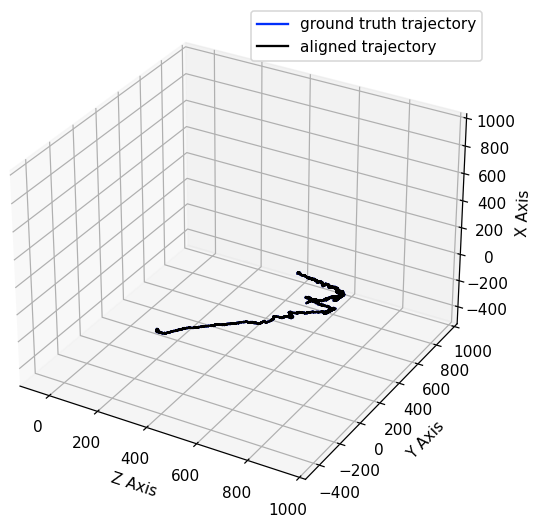
\includegraphics[width=\textwidth]{Images/48_iter_traj.png}
  \captionof{figure}{Ground truth and estimated aligned trajectories}
  \label{fig:iterative_traj_48}
\end{minipage}%
\begin{minipage}{.45\textwidth}
  \centering
  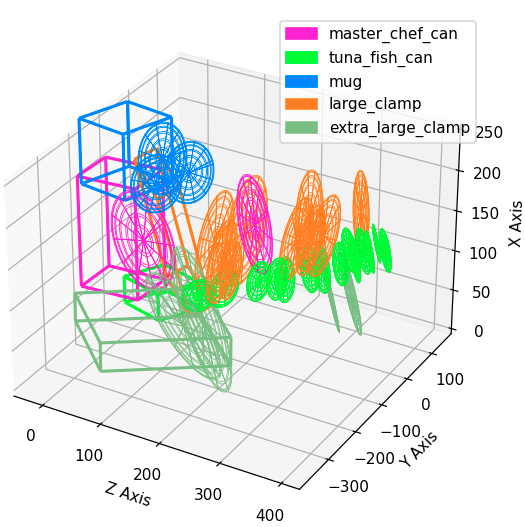
\includegraphics[width=\textwidth]{Images/48_iter_quads.png}
  \captionof{figure}{Ground truth and estimated object pose}
  \label{fig:iterative_obj_48}
\end{minipage}
\end{figure}
\item The above plots show the QuadricSLAM qualitative performance when the iterative optimization option is turned ON.
    \item In figure\ref{fig:iterative_48}, the trajectory and the object poses are plotted. The B,G,R colors of the quiver axis of the trajectory corresponds to X,Y,Z axis direction. So in this case, the red arrows are pointed towards the objects. The objects are plotted as ellipsoids. We can see there are duplicate instances of the same object even though only 1 object of each class was present in the scene.
    \item In figure\ref{fig:ground_truth_48}, the ground truth trajectory is plotted along with the ground truth objects. The YCB object model is used to find the length, width and height of the object which is used to plot the 3D box here.
    \item In figure\ref{fig:iterative_traj_48}, we can see that the ground truth trajectory and the estimated trajectory are aligning as the noise model is less noisy.
    \item In figure\ref{fig:iterative_obj_48}, the ground truth object is represented as 3D boxes and the estimated object poses are represented as ellipsoids. We can see that there is association problem existing causing duplication of objects.
    \item We can see that the objects are getting duplicated over time. This is due to the fact that in each optimization step, the camera poses and the object dual quadric matrix are jointly corrected. This causes the camera poses to deviate heavily to correct the object pose error even though we provide accurate camera poses to the SLAM system by passing the ground truth trajectory. So in the next upcoming steps, the camera assumes to view the same object at a different object pose causing a duplication of the same object. This experiment shows the necessity of a more robust and stable feature detector to run in the backend to estimate the camera pose and object pose accurately which is solved by OA-SLAM which has ORB feature tracking based ORB-SLAM2 running in the backend.
\end{itemize}

\subsubsection{Batch optimization}
\begin{itemize}
\begin{figure}[H]
\centering
\begin{minipage}{.45\textwidth}
  \centering
  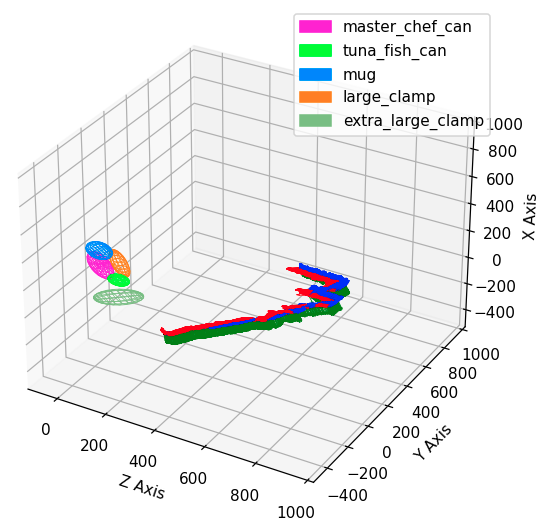
\includegraphics[width=\textwidth]{Images/48_batch_complete.png}
  \captionof{figure}{Batch optimized trajectory and object ellipsoids}
  \label{fig:batch_48}
\end{minipage}%
\begin{minipage}{.45\textwidth}
  \centering
  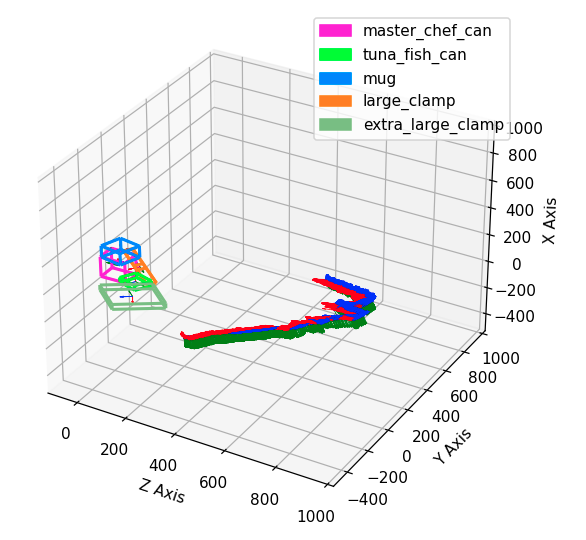
\includegraphics[width=\textwidth]{Images/48_gt_traj_box.png}
  \captionof{figure}{Ground truth trajectory and object 3D box}
  \label{fig:gt_48}
\end{minipage}
\end{figure}

\begin{figure}[H]
\centering
\begin{minipage}{.45\textwidth}
  \centering
  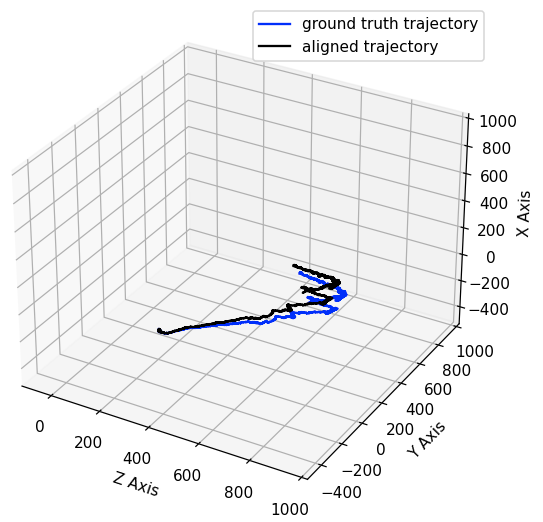
\includegraphics[width=\textwidth]{Images/48_batch_traj.png}
  \captionof{figure}{Ground truth and estimated aligned trajectories}
  \label{fig:batch_traj_48}
\end{minipage}%
\begin{minipage}{.45\textwidth}
  \centering
  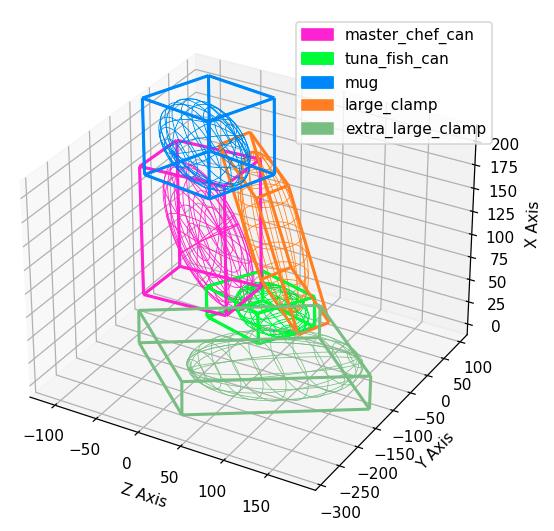
\includegraphics[width=\textwidth]{Images/48_batch_obj.png}
  \captionof{figure}{Ground truth and estimated object pose}
  \label{fig:batch_obj_48}
\end{minipage}
\end{figure}

    \item The above plots depict the QuadricSLAM qualitative performance when the batch optimization option is turned ON.
    \item In figure\ref{fig:batch_48}, we can see the trajectory pattern and the object poses are similar to what is expected in figure\ref{fig:gt_48} which is the ground truth.
    \item In figure\ref{fig:batch_traj_48}, we can see that the trajectories are similar in pattern, but an alignment error accumulates over time.
    \item In figure\ref{fig:batch_obj_48}, the 3D ground truth boxes and the estimated object ellipsoids are well overlapping. There are no association or duplication issues.
    
    \item In cases where we need to test the mapping capability of the SLAM system, we can use the ground truth trajectory and add it to the factor graph with noise model as zero. This makes the odometry variable unmodifiable in the factor graph. This implementation is used to visualize the QuadricSLAM performance for object mapping given the exact camera pose. In such case, the estimated trajectory would align with the ground truth trajectory as in figure\ref{fig:iterative_traj_48}.
    \end{itemize}



    \section{Results}

    Describe the results of your experiments in detail.
    \begin{itemize}
        \item All the plots, pictures, tables
        \item Rainfall plot
    \end{itemize}
    \begin{itemize}
    
    
    

    \item \textbf{EVALUATION METRICES}
    \item \textbf{Object pose errors}
        
\begin{table}[htbp]
    \centering
    \begin{tabular}{|c|c|c|}  % Use 'c' for centered columns, '|' for vertical lines
        \hline  % Horizontal line
        Class name & Euclidean error(mm) & Rotation error(rad)  \\  % Header row
        \hline  % Horizontal line
        master chef can & 38.656 & 2.187 \\
        tuna fish can & 40.259 & 1.417 \\
        mug & 31.222 & 1.815 \\
        large clamp & 16.719 & 1.850 \\
        extra large clamp & 73.906 & 2.043 \\
        \hline  % Horizontal line
    \end{tabular}
    \caption{Object pose errors}
    \label{tab:Object_pose_errors}
\end{table}
The Root Mean Square Error is the average of all the Euclidean errors which is \textbf{40.153 mm}.
The average rotation error is \textbf{1.862 radians}.

\item \textbf{Object Overlapping Volume Error}
\begin{table}[htbp]
    \centering
    \begin{tabular}{|c|c|}  % Use 'c' for centered columns, '|' for vertical lines
        \hline  % Horizontal line
        Class name & Overlap(\%)\\  % Header row
        \hline  % Horizontal line
        master chef can & 24.37 \\
        tuna fish can & 24.90 \\
        mug & 48.80 \\
        large clamp & 67.57 \\
        extra large clamp & 16.32 \\
        \hline  % Horizontal line
    \end{tabular}
    \caption{Object Overlapping Percentage}
    \label{tab:Object_Volume_Error}
\end{table}

The average overlapping between ground truth cuboid and estimated ellipsoids is \textbf{36.39\%}. The higher the volume, the better the overlapping. To increase the accuracy of overlapping checking, increase the number of Monte Carlo samples being generated.

    \item \textbf{Camera pose or trajectory errors}
    \begin{itemize}
        \item \textbf{Trajectory deviation error}
\begin{figure}[H]
\centering
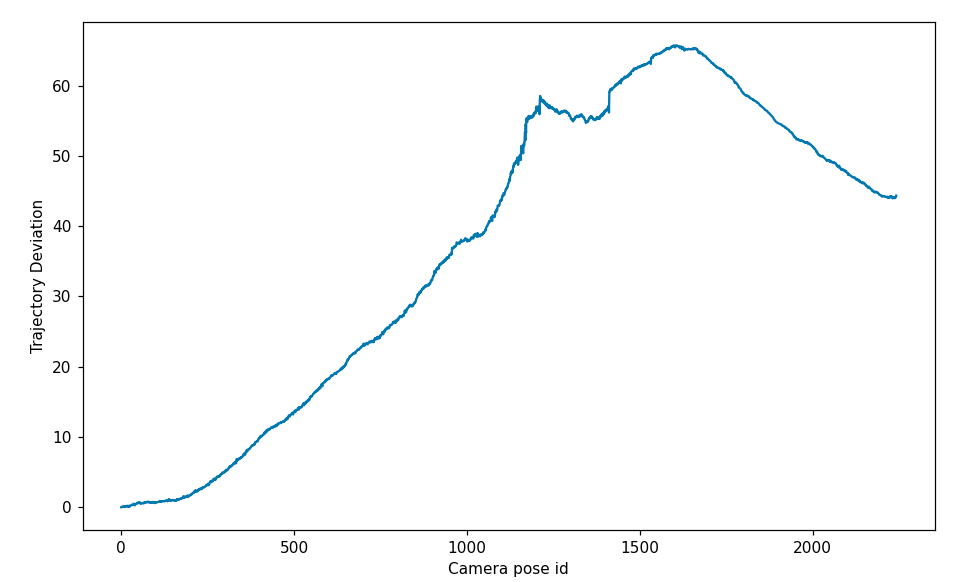
\includegraphics[width=0.8\textwidth] {Images/traj_deviation.png}
\caption{\centering Trajectory Deviation Error}
\label{fig:Trajectory_Deviation_Error}
\end{figure}
The above figure shows the growth of the trajectory deviation over time. Initially, the deviation was around \textbf{0 mm} and later reached a maximum deviation of \textbf{65.727 mm}. The Root Mean Square Error(RMSE) is \textbf{36.922 mm}.
        \item \textbf{Rotation error}
\begin{figure}[H]
\centering
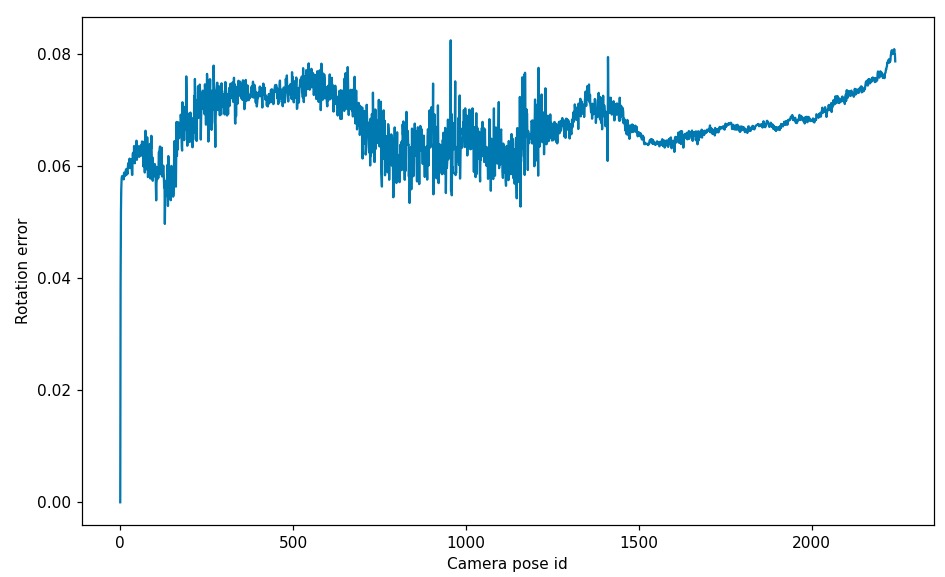
\includegraphics[width=0.8\textwidth] {Images/rot_error.png}
\caption{\centering Rotation Error}
\label{fig:Rotation_Error}
\end{figure}
The above figure shows the growth of the rotation error over time. The average rotation error is \textbf{0.067 radians}. The minimum rotation error is \textbf{0 radians} and the maximum rotation error is \textbf{0.082 radians}.
    \end{itemize}
    \item \textbf{Procrustes Analysis} - The estimated disparity value is \textbf{0.000235}. Procrustes analysis tries to align two given trajectory points and minimize the distance between them. The disparity or distortion after aligning is returned as the disparity value which indicates a better similarity between the trajectories if the disparity value is low. 
    \item \textbf{Fréchet Distance} - The estimated Fréchet Distance is \textbf{65.298 mm}. Fréchet Distance takes the shape of the trajectory curve along with its temporal feature to identify the length of the minimum leash distance that can connect two similar points of each trajectory. It is similar to dynamic time warping.  A lower Fréchet Distance indicates more correlation or similarity between the two trajectory curves and a higher Fréchet Distance indicates dissimilarity. This value is similar to the maximum trajectory deviation value.
    \item \textbf{Chamfer Distance} - The estimated Chamfer Distance is \textbf{62.787 mm}. Chamfer Distance is a symmetric matrix as it computes the Euclidean distance of a point in one trajectory to the neighbouring point in the other trajectory and vice versa. The Chamfer Distance indicates the alignment distance required to make the trajectories similar. Lower Chamfer Distance indicates better similarity.
    \item \textbf{Uninitiated objects error} - The value is 0 as all objects got initiated.
    \item \textbf{Association error} - The value is 0 as all 5 objects are associated correctly.
    \item \textbf{Duplication error} - The value is 0 as there are no duplicated objects.
    \item \textbf{Size of stored map} - For the scene with 2243 camera poses and 5 objects, the file size is 690 KB. This size can further go down by removing the last row of the pose matrix which is always [0,0,0,1].
    
\end{itemize}

\begin{itemize}
    \item \textbf{RAINFALL PLOTS OF BOP YCBV TEST SCENES}


\begin{figure}[H]
\centering
\begin{minipage}{.45\textwidth}
  \centering
  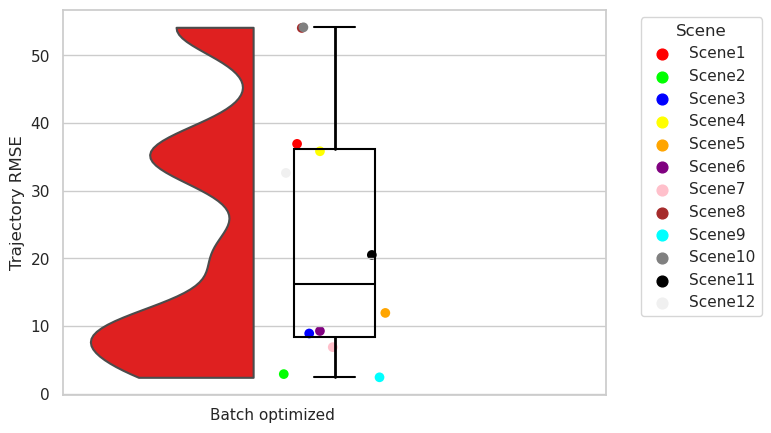
\includegraphics[scale=0.45]{Images/Trajectory_RMSE_batch.png}
  \captionof{figure}{RMSE - Batch Optimised}
  \label{fig:Trajectory_RMSE_batch.png}
\end{minipage}%
\begin{minipage}{.45\textwidth}
  \centering
  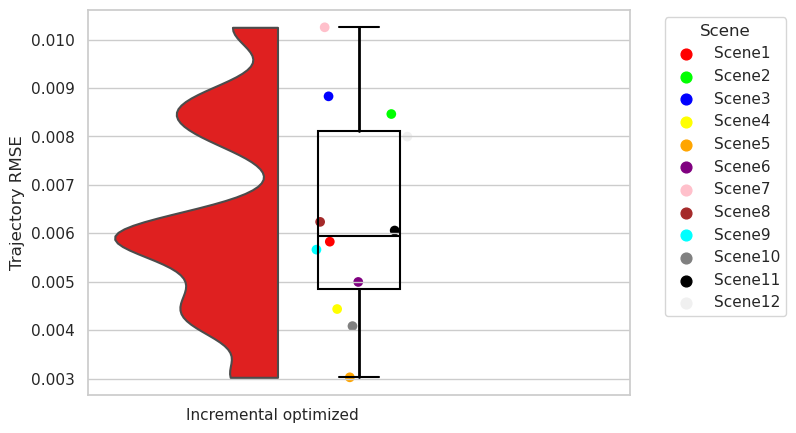
\includegraphics[scale=0.45]{Images/Trajectory_RMSE_incre.png}
  \captionof{figure}{RMSE - Incremental Optimised}
  \label{fig:Trajectory_RMSE_incre.png}
\end{minipage}
\end{figure}


\begin{figure}[H]
\centering
\begin{minipage}{.45\textwidth}
  \centering
  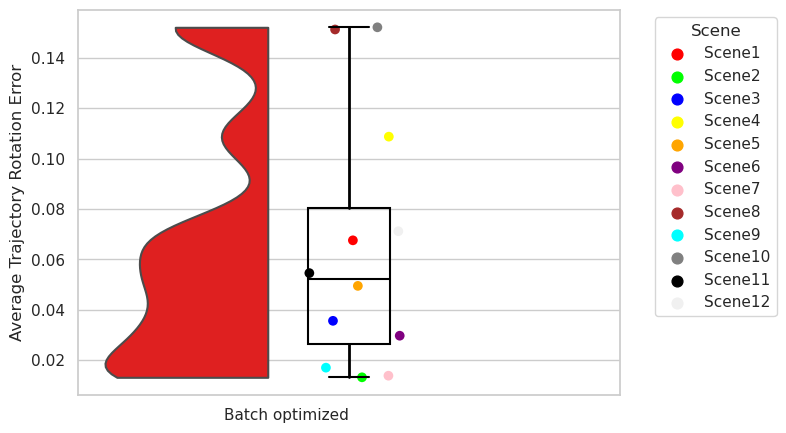
\includegraphics[scale=0.45]{Images/Average_Trajectory_Rotation_Error_batch.png}
  \captionof{figure}{\begin{varwidth}{0.6\textwidth}Average Trajectory Rotation Error - Batch Optimised\end{varwidth}}
  \label{fig:Average_Trajectory_Rotation_Error_batch.png}
\end{minipage}%
\begin{minipage}{.45\textwidth}
  \centering
  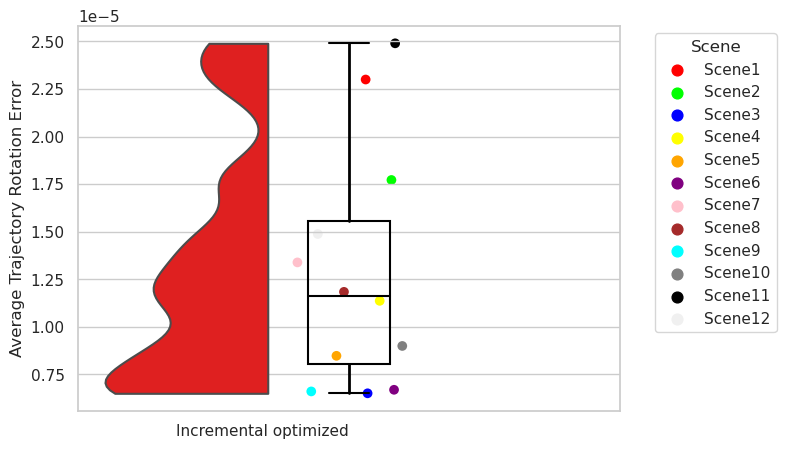
\includegraphics[scale=0.45]{Images/Average_Trajectory_Rotation_Error_incre.png}
  \captionof{figure}{\begin{varwidth}{0.6\textwidth}Average Trajectory Rotation Error - Incremental Optimised\end{varwidth}}
  \label{fig:Average_Trajectory_Rotation_Error_incre.png}
\end{minipage}
\end{figure}



\begin{figure}[H]
\centering
\begin{minipage}{.45\textwidth}
  \centering
  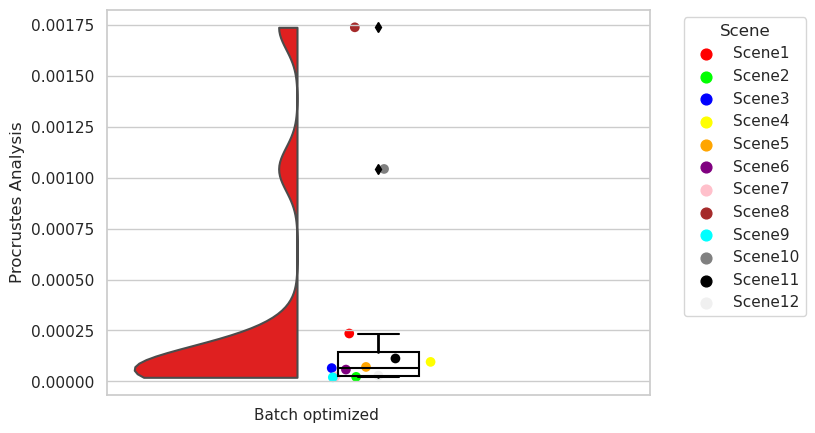
\includegraphics[scale=0.45]{Images/Procrustes_Analysis_batch.png}
  \captionof{figure}{\begin{varwidth}{0.6\textwidth}Procrustes Analysis - Batch Optimised\end{varwidth}}
  \label{fig:Procrustes_Analysis_batch.png}
\end{minipage}%
\begin{minipage}{.45\textwidth}
  \centering
  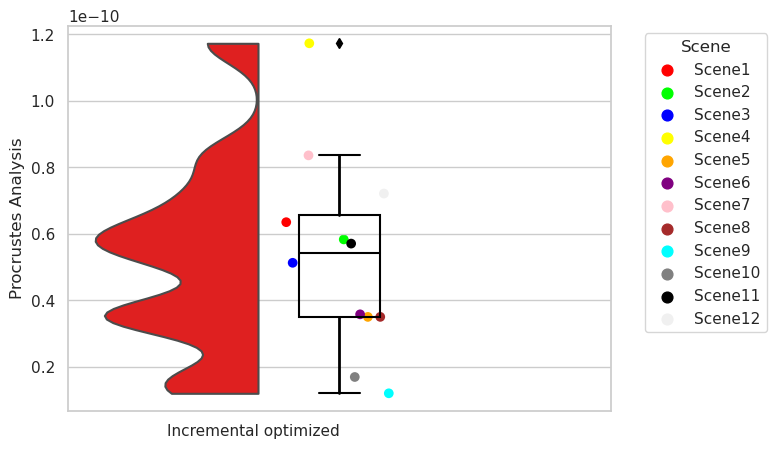
\includegraphics[scale=0.45]{Images/Procrustes_Analysis_incre.png}
  \captionof{figure}{\begin{varwidth}{0.6\textwidth}Procrustes Analysis - Incremental Optimised\end{varwidth}}
  \label{fig:Procrustes_Analysis_incre.png}
\end{minipage}
\end{figure}


\begin{figure}[H]
\centering
\begin{minipage}{.45\textwidth}
  \centering
  \includegraphics[scale=0.45]{Images/Fréchet_Distance_batch.png}
  \captionof{figure}{\begin{varwidth}{0.6\textwidth}Fréchet Distance - Batch Optimised\end{varwidth}}
  \label{fig:Fréchet_Distance_batch.png}
\end{minipage}%
\begin{minipage}{.45\textwidth}
  \centering
  \includegraphics[scale=0.45]{Images/Fréchet_Distance_incre.png}
  \captionof{figure}{\begin{varwidth}{0.6\textwidth}Fréchet Distance - Incremental Optimised\end{varwidth}}
  \label{fig:Fréchet_Distance_incre.png}
\end{minipage}
\end{figure}


\begin{figure}[H]
\centering
\begin{minipage}{.45\textwidth}
  \centering
  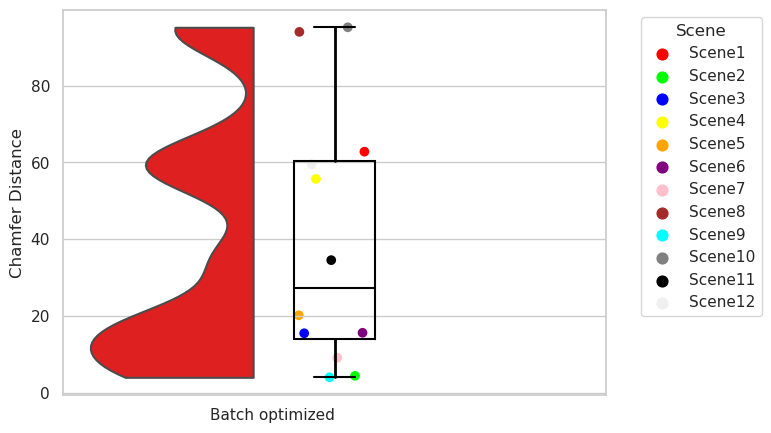
\includegraphics[scale=0.45]{Images/Chamfer_Distance_batch.png}
  \captionof{figure}{\begin{varwidth}{0.6\textwidth}Chamfer Distance - Batch Optimised\end{varwidth}}
  \label{fig:Chamfer_Distance_batch.png}
\end{minipage}%
\begin{minipage}{.45\textwidth}
  \centering
  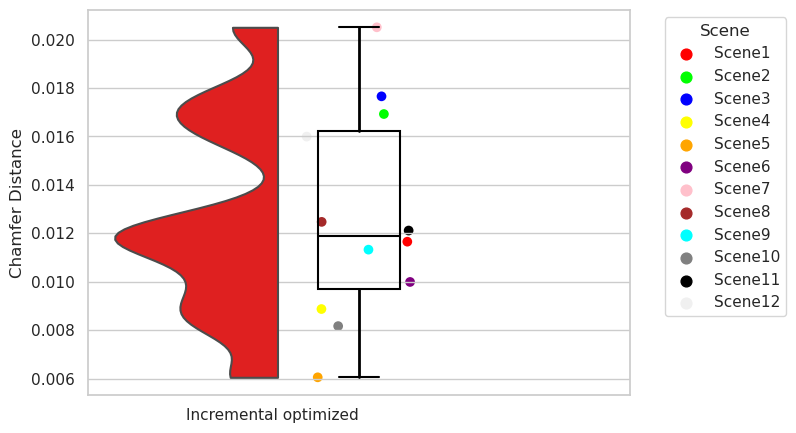
\includegraphics[scale=0.45]{Images/Chamfer_Distance_incre.png}
  \captionof{figure}{\begin{varwidth}{0.6\textwidth}Chamfer Distance - Incremental Optimised\end{varwidth}}
  \label{fig:Chamfer_Distance_incre.png}
\end{minipage}
\end{figure}


\begin{figure}[H]
\centering
\begin{minipage}{.45\textwidth}
  \centering
  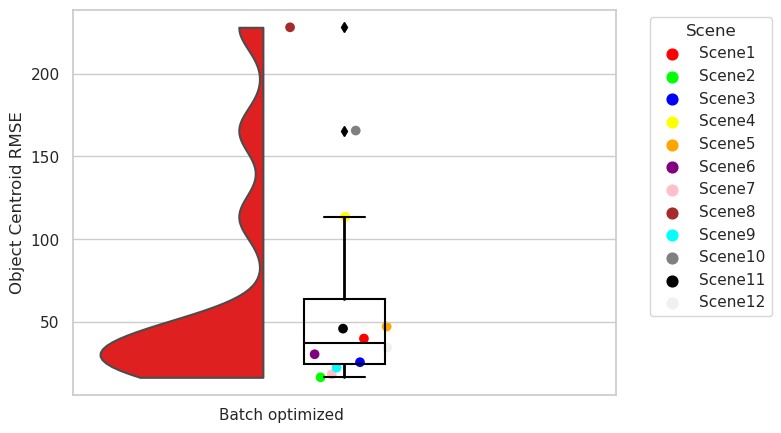
\includegraphics[scale=0.45]{Images/Object_Centroid_RMSE.png}
  \captionof{figure}{\begin{varwidth}{0.6\textwidth}Object Centroid RMSE - Batch Optimised\end{varwidth}}
  \label{fig:Object_Centroid_RMSE.png}
\end{minipage}
\begin{minipage}{.45\textwidth}
  \centering
  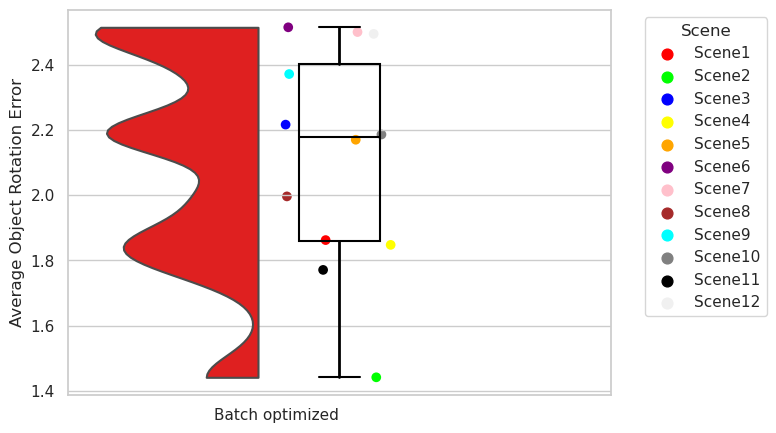
\includegraphics[scale=0.45]{Images/Average_Object_Rotation_Error.png}
  \captionof{figure}{\begin{varwidth}{0.6\textwidth}Average Object Rotation Error - Batch Optimised\end{varwidth}}
  \label{fig:Average_Object_Rotation_Error.png}
\end{minipage}%
\end{figure}


\begin{figure}[H]
\centering
\begin{minipage}{.45\textwidth}
  \centering
  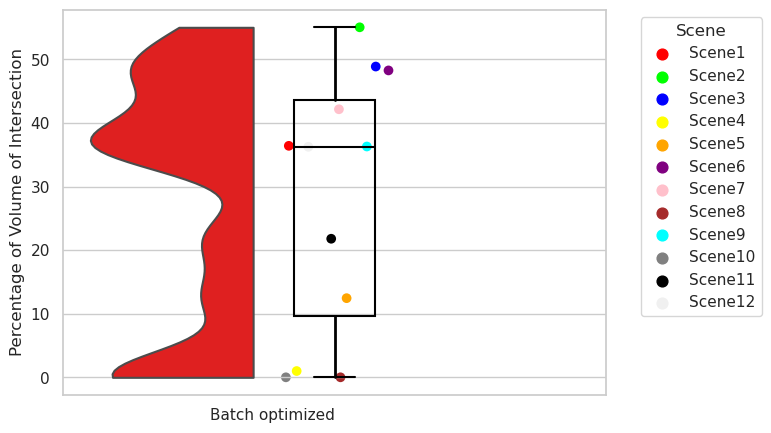
\includegraphics[scale=0.45]{Images/Percentage_of_Volume_of_Intersection.png}
  \captionof{figure}{\begin{varwidth}{0.6\textwidth}Percentage of Volume of Intersection - Batch Optimised\end{varwidth}}
  \label{fig:Percentage_of_Volume_of_Intersection.png}
\end{minipage}

\end{figure}

    
\end{itemize}

\end{document}
